%% Karlsruhe Institute of Technology
%% Institute for Anthropomatics and Robotics (IAR)
%% Artificial Intelligence for Language Technologies (AI4LT) lab
%%
%% Prof. Dr. Jan Niehues
%% Lab's website https://ai4lt.anthropomatik.kit.edu/english/index.php

\iflanguage{english}
{\chapter{Appendix}}    % english style
{\chapter{Anhang}}      % german style
\label{chap:appendix}
\section{Implementation information}\label{ch:implementation information}
Following more in depth information about how exactly the probabilities are retrieved with the help of huggingface models and pytorch. 
\subsection{transcription probability}
To retrieve the final transcription probability the huggingface model of whisper returns a tuple (or dictionary) that contains the probability of each vocabulary entry at each decoding step.
Those values are then processed so that the sum of the highest probabilities is taken and then normalised by the number of decoding steps that were done, this gives the transcription probability mean. For reference the pure probability sum was also collected and returned during the experiments. 
There is a small difference in the resulting QE scores between the two versions but that is more noticeable in the dropout version of the transcription probability 

\subsection{Translation probability}
To get the probability of the top token at each decoding step the functionality from huggingface is used, which is able to return the log-probabilities and scores, so the processed log-probability, of all vocabulary entries. 
Then to get the final probability of the sequence the top token of each decoding step and it's probability is picked and the then summed up and divided by the number of decoding steps that are in the sequence.

\subsection{Softmax entropy}
To get the vocabulary values at each decoding stem from the seamless model basic code has been written that iterates over all vocabulary tokens, which are returned by the model generation by the huggingface model and calculated the entropy of each decoding step.

To get them from DeltaLm the fairseq source code was adapted to do the same as the huggingface model, namely return the probability of all tokens, as the fairseq toolkit is unable to do so natively so far.
But due to how the fairseq toolkit returns information the sum of the softmax entropy over the vocabulary at each decoding step was actually returned. 

In the Formicheva \cite{fomicheva2020unsupervised} paper the Softmax entropy measure was proposed as $$-\frac{1}{T}\sum_{t=1}^T\sum_{v=1}^Vp(y_t^v)logp(y_t^v)$$ with V being the Vocabulary size and T being the length of the translation. Which in this definition doesn't work with the data that the models produce as there are quite a lot of 0 values for the vocabulary after using the softmax, which means that the result of the sum like that would not be defined, as the log of 0 is undefined but approaches $-\infty$. To mitigate this the 0 values are masked for the log and by extend the sum, so those values are essentially ignored. 

\subsection{Standard deviation }
The standard deviation is calculated over the top token probability at each decoding step. 
Those probabilities are the same ones that are retrieved in the translation probability part.
On those results the numpy implementations of the standard deviation\cite{numpystddiv} was then used to retrieve the score.

On DeltaLM it's done with the help of the numpy implementation on the probabilities that have been output by fairseq. 
The numpy implementation of the standard deviation takes an array like data structure and if it is not given, calculates the mean of the values in the array and then with that the deviation of the values from the mean. 
The standard deviation used in numpy is defined as $$\sqrt{\frac{\sum_i |a_i-\overline{a}|}{N}}$$ where $\overline{a}$ is the mean and $a_i$ is the i-th element in the array.
%% -------------------
%% | Example content |
%% -------------------

\section{Other interesting pearson correlation scores}\label{dropout softmax entropy}

The pearson correlation of the entropies in dropout shows a significant prediction value with a correlation of the mean of -0.23241 and 0.29450, and a correlation of -0.17032 and - 0.12806 of the variance of the entropies on seamless and DeltaLM respectively. Which is higher than just the regular translation probability and variance but it comes with a significant cost to compute as calculating the softmax entropy is very rarely implemented in frameworks.


 
  
 
  
  
 


\section{references graphs}
\label{sec:appendix:FirstSection}
Since there are a lot of plots that contain plots over the reference scores it might be intersting to see how those references fall over the data set. 

\setcounter{figure}{0}

\begin{figure}[ht]
    \centering
    \begin{subfigure}{0.7\textwidth}
    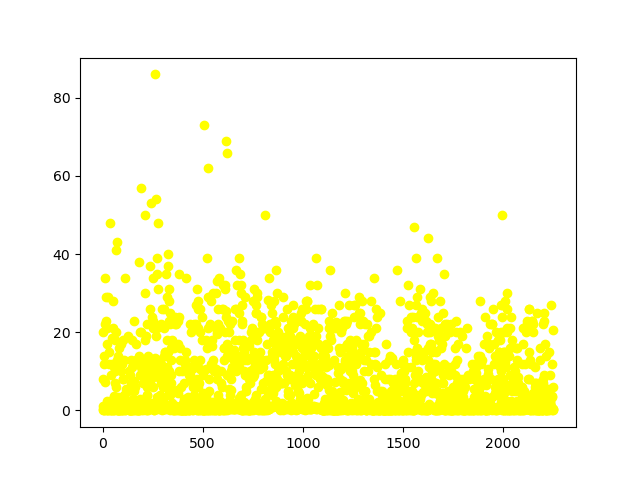
\includegraphics[width=\linewidth]{Latex/sections/images/seamlesswerref.png}
    \caption{all of the reference scores of the dataset, the x axis is the lines in teh dataset, the y axis is the WER scores}
    \end{subfigure}
    \begin{subfigure}{0.7\textwidth}
        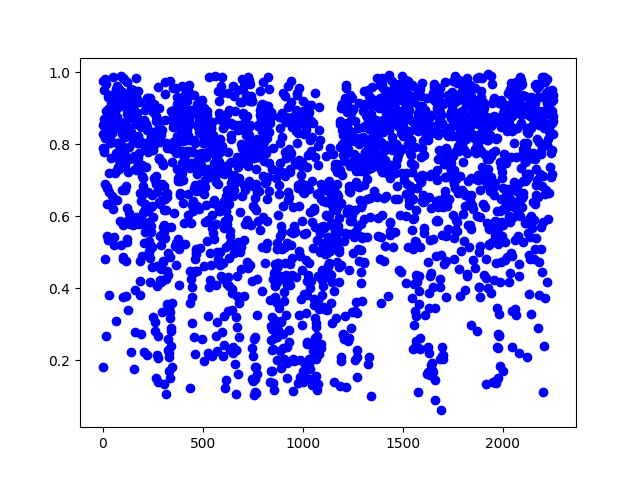
\includegraphics[width=\linewidth]{Latex/sections/images/seamlessreferences.png}
        \caption{refrence coment scores from seamless}
    \end{subfigure}
    \label{fig:reference scatterplot}
\end{figure}



%% ---------------------
%% | / Example content |
%% ---------------------